\section{Aufbau und Durchführung}
\label{sec:Durchführung}

Der Versuchsaufbau ist in \autoref{fig:Abb_4} dargestellt.
\begin{figure}[H]
    \centering
    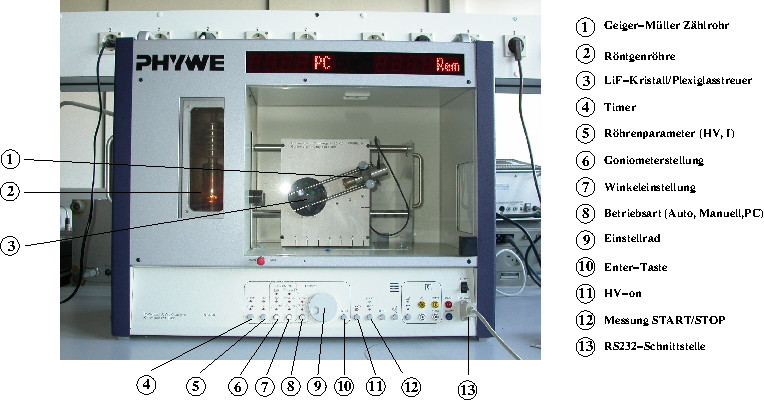
\includegraphics[width=\textwidth]{build/Abb_4.pdf}
    \caption{Versuchsaufbau und Benennung der Bestandteile.\cite{V602}}
    \label{fig:Abb_4}
\end{figure}

Die wesentlichen Bestandteile sind eine Kupfer-Röntgenröhre, ein LiF-Kristall und ein Geiger-Müller-Zählrohr.
Die Strahlung der Röntgenröhre ist auf den Kristall gerichtet, wobei dieser drehbar ist und somit die Intensität der 
Röntgenstrahlung durch das Geiger-Müller-Zählrohr für variierbare Glanzwinkel gemessen werden kann.
Mithilfe der Einstellelemente der Apparatur kann die Messung geregelt werden. Die Beschleunigungsspannung an der Röntgenröhre
wird für alle Messungen auf $U = \qty{35}{\kilo\volt}$ eingestellt und der Emissionsstrom am Geiger-Müller-Zählrohr auf $I = \qty{1}{\milli\ampere}$.
Mithilfe der Winkeleinstellung ($7$) kann ein fester Winkel für den LiF-Kristall eingestellt werden.
Die $\qty{1}{\milli\meter}$ Blende und der Kristall werden in die jeweiligen Halterungen gebracht.
Die Schlitzblende muss waagerecht auf dem Geiger-Müller-Zählrohr sitzen.
Die Messergebnisse werden über einen PC aufgenommen. 
Es kann die Messart, der Kristallwinkel, ein Drehmodus und die Integrationszeit für die Messungen ausgewählt bzw. eingestellt werden.
Als Messart wird  \enquote{Spektren} verwendet.

\subsection{Überprüfung der Bragg-Bedingung} % (fold)
\label{sub:Bragg_durch}

Im ersten Versuchsteil wird die Bragg-Bedingung überprüft. Dazu wird ein fester Kristallwinkel von $\theta = \qty{14}{\degree}$ eingestellt.
Mit einem Winkelzuwachs von $\Delta\theta = \qty{0.1}{\degree}$ in einer Integrationszeit
von $\Delta t = \qty{5}{\second}$ wird die Intensität der Röntgenstrahlung am Geiger-Müller-Zählrohr in
einem Winkelbereich von $\theta_{GM} = \qty{26}{\degree}$ bis $\theta_{GM} = \qty{30}{\degree}$ gemessen.
Es wird eine Funktion der Zählrate gegenüber des Kristallwinkels geplottet und das Maximum der Kurve bestimmt.
% subsection Überprüfung der Bragg-Bedingung (end)

\subsection{Analyse des Emissionsspektrums einer Cu-Röntgenröhre} % (fold)
\label{sub:Emission_durch}

Um das Emissionsspektrum der Röntgenröhre aufzunehmen werden im Programm measure die Einstellungen verändert.
Die Messung erfolgt im 2:1 Koppelmodus. Das Röntgenspektrum wird im Winkelbereich von $\theta = \qty{4}{\degree}$ bis $\theta_{GM} = \qty{26}{\degree}$ gemessen. 
Der Winkelzuwachs wird auf $\Delta\theta = \qty{0.2}{\degree}$ und die Integrationszeit wird beibehalten.
Auch hier wird eine Funktion der Zählrate gegnüber dem Kristallwinkel geplottet und die Maxima bestimmt.
Anschließend wird die Halbwertsbreite bestimmt und daraus das Auflösungsvermögen der Apparatur.
Zuletzt werden die Abschirmkonstanten von Kupfer aus den Emmissionsenergien der $K_{\alpha}$- und $K_{\beta}$-Linien.

% subsection Das Emissionsspektrum einer Cu-Röntgenröhre (end)

\subsection{Analyse der Absorptionsspektren} % (fold)
\label{sub:Absorption_durch}
Um das Absorptionsspektrum zu messen wird ein Absorber vor das Geiger-Müller Zählrohr gesetzt.
Der Winkelzuwachs wird wieder auf $\Delta\theta = \qty{0.1}{\degree}$ eingestellt und die Integrationszeit
auf $\Delta t = \qty{20}{\second}$ erhöht. Der Messbereich ist abhängig von dem Absorber und muss somit individuell angepasst werden.
Aus der geplotten Funktion wird die Absorptionsenergie der gemessenen K-Kante bestimmt.
Anschließend wird die Abschirmzahl $\sigma_K$ berechnet.
Diese Messung wird für insgesamt für fünf Absorber durchgeführt.
Die Abschirmzahlen wird aus den bestimmten Energieübergängen  aus den gemessenen K-Kanten berechnet.
Zuletzt wird aus den bestimmten Absorberenergien eine $\sqrt{E_K}-Z$ Diagramm gezeichnet und aus der Steigung
die Rydbergkonstante berechnet.

% subsection Das Absorptionsspektrum (end)